\documentclass{article} % For LaTeX2e
%\documentstyle[nips12submit_09,times,art10]{article} % For LaTeX 2.09
\usepackage{nips12submit_e,times,graphicx}
\usepackage{epstopdf}
\nipsfinaltrue

\newcommand{\floe}{\emph{Floe }}

\graphicspath{{./figures/}}
\DeclareGraphicsExtensions{.eps}

\title{Distributed Online Clustering using LSH over Multiple Data Streams}

\author{
Alok Kumbhare \\
Department of Computer Science \\
University of Southern California \\
Los Angeles, CA 90007 \\
\texttt{kumbhare@usc.edu} \\
\And
Ketan Singh \\
Department of Computer Science \\
University of Southern California \\
Los Angeles, CA 90007 \\
\texttt{ketansin@usc.edu} \\
}

% The \author macro works with any number of authors. There are two commands
% used to separate the names and addresses of multiple authors: \And and \AND.
%
% Using \And between authors leaves it to \LaTeX{} to determine where to break
% the lines. Using \AND forces a linebreak at that point. So, if \LaTeX{}
% puts 3 of 4 authors names on the first line, and the last on the second
% line, try using \AND instead of \And before the third author name.

\newcommand{\fix}{\marginpar{FIX}}
\newcommand{\new}{\marginpar{NEW}}

\begin{document}


\maketitle

\section{Abstract}

\section{Introduction}
Terabytes of data is being generated by social networks. There are 250 millions of tweets coming up every day with an average of 3000 tweets per second  with variable data rates ranging from 2000 to 25,000 tweets per second. Similar data streams are available from a number of other social networks including Google +, Facebook, Quora, etc.  Aggregating data from all these social networks will provide data messages with even higher data rates. 

Data analysts use these streams for various applications including trend analysis, recommender systems, advertisement placements, sentiment analysis etc. Each of these data streams contain a mix of topics, but, most of these applications require data clustered on certain criterion for processing. For example, sentiment analysis applications are usually dedicated towards gauging the overall sentiment for a particular person, event, or an object. Hence it would only need access to the data items from the stream related to that topic and all other data items would only contribute towards noise. In addition, performing sentiment analysis across various social networks would provide a better  estimate on the perceived  sentiment than using only data stream from a single network.

This problem is similar to the similarity search problem in data mining which is responsible for retrieving a set of data objects similar to a given query object. The traditional similarity search algorithm has been used in a variety of domains with applications ranging from de-duplication, content based search for audio, video, and images, pattern classification, natural language processing, clustering and many others. 

In most of these applications the objects are represented by high dimensional feature vector. A large static collection of such data objects is stored in a repository. Given a single (or a batch of) query object(s), the goal is to find the set of objects closes to each of the query objects that are present in the repository. Various indexing schemes have been proposed to allow efficient search of such data objects in the repository. In addition, the data archived by such applications is inherently distributed in nature and a centralized indexing scheme requires unnecessary data transfer between the data nodes. Hence a distributed indexing scheme is desired which can delegate the search operations to individual nodes in the distributed environment which will drastically reduce the data transfer requirements and hence increase efficiency.

Locality Sensitive Hashing (LSH) is one of the most efficient family of models used for similarity searching that has been shown to scale well for high dimensional data. The simple implementation of LSH requires large number of buckets to be created to achieve acceptable search quality, however, this has been mitigated by the Entropy LSH scheme which makes it suitable candidate for distributed implementation [5]. Bahmani et. al. uses Entropy LSH as the basis for an efficient implementation of the distributed Locality Sensitive Hashing to perform similarity search over high dimensional data.

The problem of generating topic streams can be solved using LSH as the core subroutine of the algorithm. However, it differs from the traditional similarity search problems in key aspects. For example, in contrast to the traditional similarity search algorithm, we do not need to find the exact match for the given query, instead it suffices to find the bucket in which the probability of obtaining a match is highest. Hence we can further optimize the LSH scheme to better suite our requirements.

In this paper, we propose an extension to the LSH scheme to be used in a distributed setting and use it as a basis for classifying incoming data items into appropriate streams. The rest of the paper is structured as follows. Section \ref{sec:LSH} discusses the traditional LSH scheme for similarity searching. We present a summary of the execution platform - FLOE - in section \ref{sec:floe}. Section \ref{sec:design} presents the proposed extension to the LSH scheme and the overall system design. We discuss preliminary results in section \ref{sec:results} followed by the planned work for the rest of the semester in \ref{sec:future}.


\section{Related Work}
\label{sec:related}
A lot of work has been done in the area of online stream clustering. [5] points out the requirements of clustering algorithms for data streams:
\begin{enumerate}
\item Compactness of representation.
\item Fast, incremental processing of new data points.
\item Clear and fast identification of "outliers".
\end{enumerate}
Data points arrive continuously in a stream. This needs to be put into appropriate cluster when it arrives. We need a compact representation of clusters because our number of clusters may easily get out of bounds of memory when new data arrives. Also there is need for fast processing of the streaming data. Otherwise, the data may easily fill up buffers and become a bottleneck in the clustering process. Thirdly, there is need to identify "outliers". At any given time some points might not fit under the current clustering model our algorithm has determined so far. Thus our algorithm should be able to handle this issue.

 [6] talks about some of the challenges for clustering of streaming data. Most of the algorithms require assistant in the form of number of expected density of clusters. There is no assumption about the number of clusters in the data stream but most clustering algorithms require it to be a fixed value. Most of the streaming data is unstructured and has a huge vocabulary. This corpus of words is not limited to a single language. So, we need to handle varied high dimensional data streams in real time. There are other issues related to uncertain data in the data streams. In most of the streams the data is unstructured and we need more information to perform statistical operations. These problems are solved by using online clustering algorithms which is the focus of this paper. Locality Sensitive Hashing helps us in processing the data streams in the required amount of time.

\section{Methodology}
\section{Experiments}
\section{Conclusion}

\section{Summary of LSH}
\label{sec:LSH}
Locality Sensitive Hashing is a probabilistic technique to find similar items to a query in high dimensional data. LSH is based on the idea that if two points are close together, then they remain close after a projection operation as well. On the other hand if two points are far apart from each other they may be near to each other in some dimension but it is more likely that they are far apart. This idea can be exploited to reduce high dimensional data into lower dimensions. Input data items are hashed using a family of hash functions so that similar items are mapped to the same buckets with high probability while dissimilar items are mapped to different buckets with high probability. This family of hash functions can be defined as: \newline
A family $H = \{h: S \rightarrow U\} $ is called $ (r_1,r_2,p_1,p_2 ) $ - sensitive for $D$ if for any $ q, p \in S$
\begin{enumerate}
\item if $ p \in B(q, r_1) $ then $ Pr_H[h(q)=h(p)] \geq p_1 $
\item if $ p \notin B(q, r_2) $ then $ Pr_H[h(q)=h(p)] \leq p_2 $
\end{enumerate}

LSH has been applied to various problems in finding similarity between two documents. It can be employed to quickly find nearest neighbours in very large databases. LSH hashes the query to some number of buckets depending upon the number of hash functions used. It is upto the application which ones they search for the query within those buckets. LSH is an approximate technique in the way that instead of finding exact matches it considers the locality of points so that closer data points remain nearby in the buckets. To summarize, unlike conventional hashes that return exact matches in O(1) time, LSH uses dot products with random hash vectors quickly identify the nearest neighbours and place them in the same buckets.



\section{FLOE - distributed stream processing platform}
\label{sec:floe}
In this section, we describe the design for \textit{Floe}, a hybrid, scalable execution engine for continuous dataflow applications and how it can be leveraged for stream clustering. \textit{Floe} is under active development at USC [2] by Simmhan et. al., and the following describes the latest design and features at the time of writing this document. 

The \floe framework supports a graph based composition model to construct continuous dataflow applications. A programmer can define a reusable tasks, called Pellet, as a custom function with a set of typed input and output ports similar to the Action-Port model. The developer can then assemble several of these tasks to form a custom graph with output ports of upstream nodes connected to the compatible input ports of downstream nodes through a communication channel. Each task performs an operation on the incoming data, transforms it to the desired format and forwards the data to the downstream task. In addition, using the named input/output ports feature, the task can direct the data to a specific node in the downstream and thus achieve functionality similar to the MapReduce model.

The \floe framework takes this application graph as input along with desired resource requirements and deploys it over a distributed environment. In addition, the framework continuously monitors the application execution to determine bottlenecks and allocate additional resources at runtime and hence provides scalable operations. It does so by monitoring the incoming data rate, the input queue, the task execution latency for each of the tasks in the application. If a bottleneck is observed, the framework increases the number of parallel instances of the given task and re-distributes the incoming data with appropriate load balancing strategies.
 

%\begin{figure}
%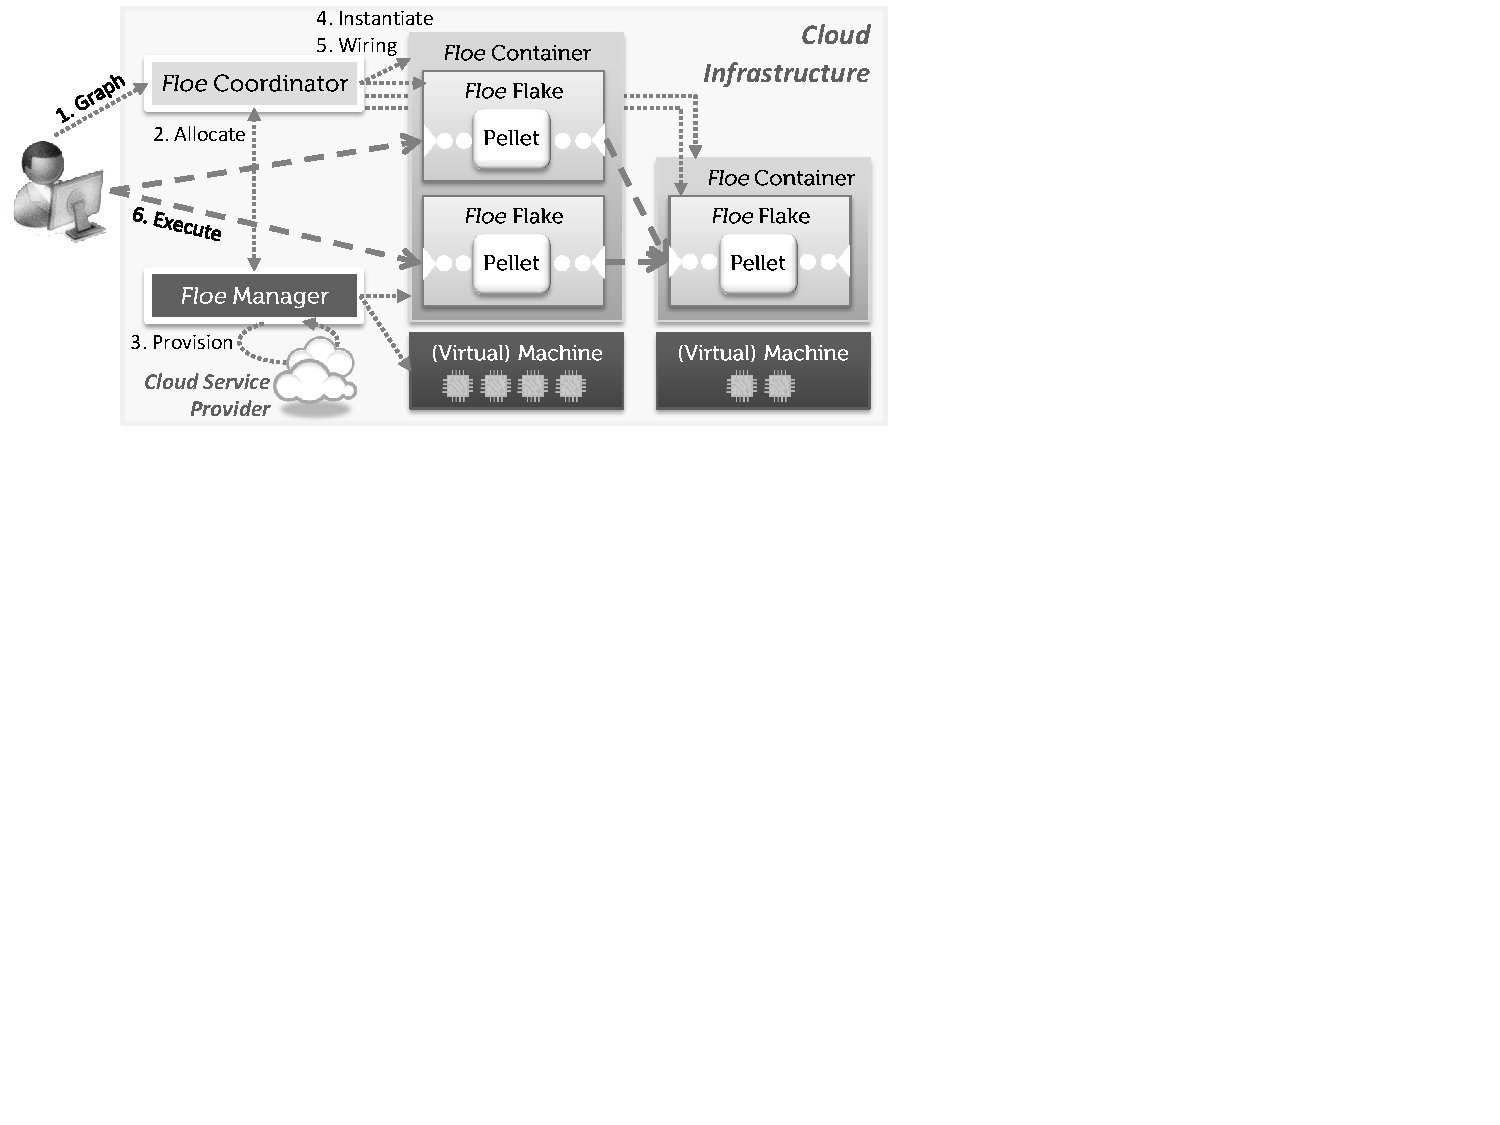
\includegraphics[width=0.5\columnwidth]{floe_arch}
%\caption{\floe Prototype Architecture}
%\label{fig:floe_arch}
%\end{figure}

\section{Stream Clustering using Distributed LSH}
\label{sec:design}
In this section, we describe the distributed LSH scheme and its application for stream clustering.

In the distributed LSH scheme, the hash buckets are distributed across various nodes in the distributed system where each node only has access to the local buckets. The buckets are distributed among the nodes using a standard hash function over the bucket id. for example using a standard mod function $Node id = Mod(bucket_{id}, \#nodes)$. This ensures equal distribution of the buckets among the distributed nodes. Note that, we do not need locality sensitive hashing to get the node id from the bucket id.

Given such a distributed system, for a given query Q, a set of $n$ hash values are obtained by running a set of locality sensitive hash functions over the query. Each of the $n$ hash values indicates the potential hash bucket (hash value is same as bucket\_id) which might contain the nearest neighbour to the given query Q. Then we hash the bucket\_id using the same standard hash function that was used for distributing buckets to obtain the node id for each of these buckets.

A message is sent to each of these nodes, with the given query Q and a list of bucket ids local to that particular node that can potentially contain the nearest neighbour for the given query Q. Each of these nodes retrieve all the data items in these potential buckets and performs a search to find the nearest neighbour and the corresponding bucket\_id. All these nodes, further send the local nearest neighbour, its distance from Q, and the bucket\_id to an aggregator node which finds the global nearest neighbor by finding the neighbour with the minimum distance among the potential candidates. Figure \ref{fig:dlsh} shows the distributed LSH scheme. 


\begin{figure}
\centering
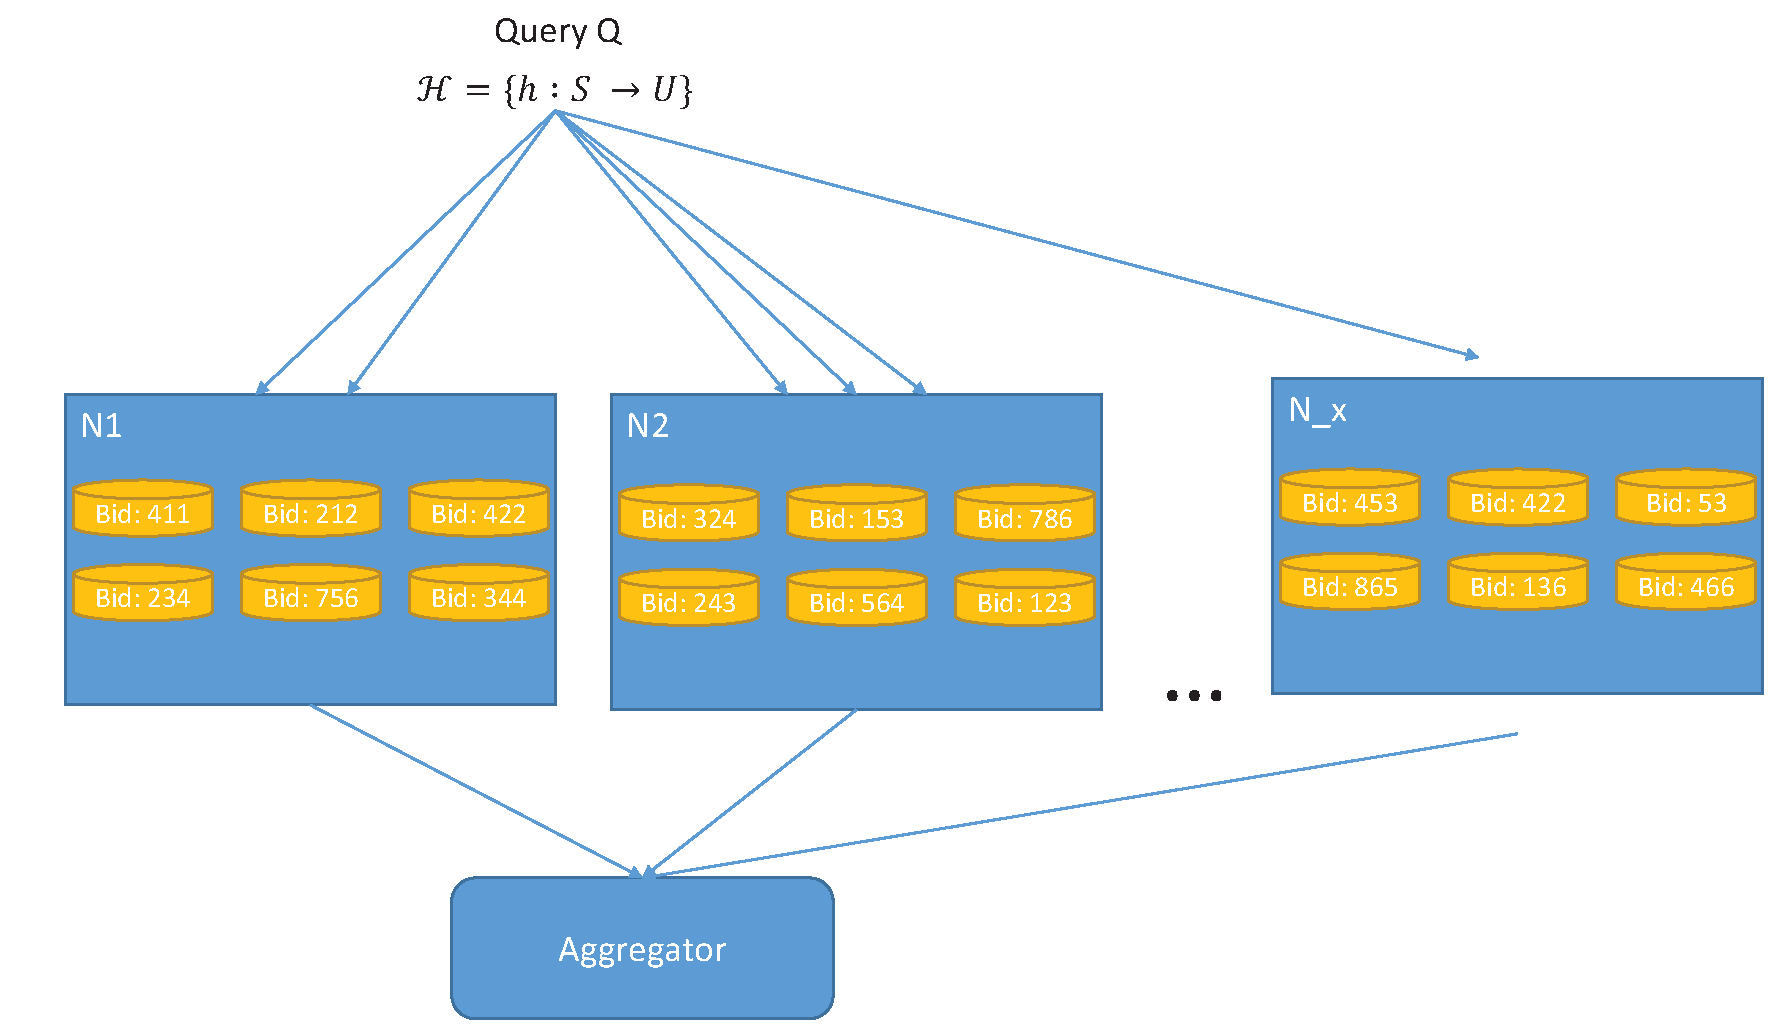
\includegraphics[width=0.8\columnwidth]{distributeLSH.pdf}
\caption{Distributed LSH Scheme}
\label{fig:dlsh}
\end{figure}



We use a variation of this distributed LSH scheme for stream clustering. Note that for stream clustering, it is not required to find the exact nearest neighbor but it is enough to find the the bucket which contains this closest neighbor. Hence, we further optimize the algorithm by keeping a representative set of data points in the bucket and compare only against these datapoints to find the bucket with the closest data point. For the preliminary investigations, we keep only a centroid of the points in the given bucket. Whenever a query is executed on this bucket, we compare only against the current centroid of the bucket for closeness and choose the bucket with minimum distance from the centroid. 

\begin{figure}{!ht}
\centering
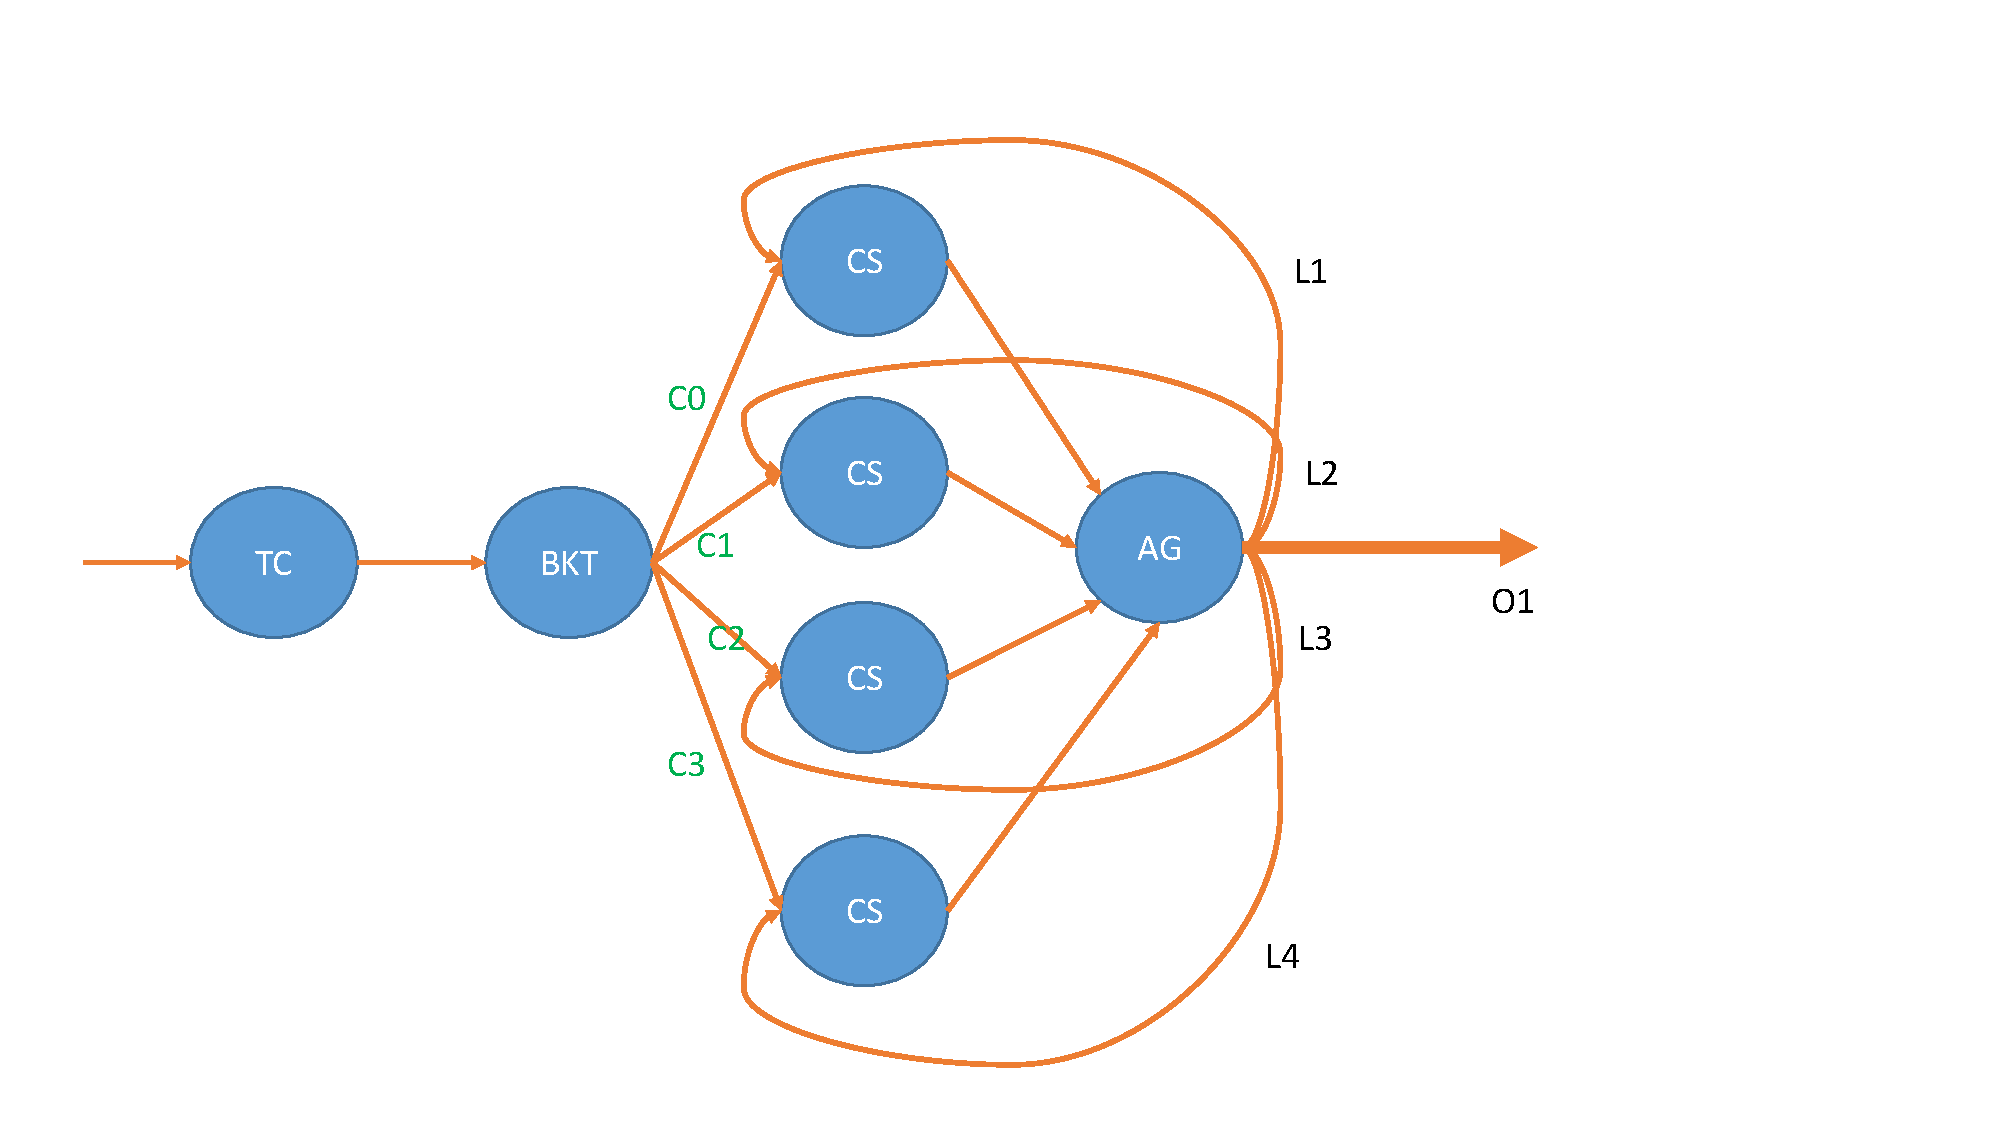
\includegraphics[width=0.8\columnwidth]{streamCluster.pdf}
\caption{Stream Clustering using Distributed LSH over FLOE framework}
\label{fig:design}
\end{figure}

Figure \ref{fig:design} shows the design for a stream classification application built using the floe framework, specialized for text streams, that we have designed using this modified distributed LSH Scheme and is described below. Each node is a Floe task connected using communication channels for transferring messages. 

\begin{enumerate}
\item Task TC ( TweetCleaner ): This task is the first one to run. It processes tweet one by one and performs tasks such as tokenization, stop word removal, stemming.
\item Task BKT ( Bucketizer ): This node extracts the features from the tweet and performs locality sensitive hashing on those features to allocate the tweet to potential clusters with high probability of match with similar tweets. It then maps these clusters ids to node ids using a predefined hash function. It also passes the list of potential clusters ids ( buckets ) to search locally at each of these nodes.
\item Task CS ( ClusterSearcher ): It receives the tweet and list of potential clusters for that tweet which has a high probability of matching. It then searches only through those clusters to find the one with the minimum Euclidean distance. This distance is calculated from the Centroid of each of the potential clusters. This process is performed at each of the nodes with their respective tweets and their list of potential clusters. Each node only has local view of the clusters and hence there is a need to aggregate the results from various nodes to get the best match across all nodes.
\item Task AG ( Aggregator ): Each of the ClusterSearcher nodes sends the local best match cluster id along with the corresponding minimum distance to the aggregator node. The aggregator node then does the second level of comparison across all these received distances to find the global minimum distance and the corresponding cluster. Based on this information the aggregator sends feedback to corresponding CS node which then updates the Centroid of that particular cluster.
\end{enumerate}





\section{Experiments and Results}
\label{sec:results}

\subsection{Data Set}
We will mainly be using the data set from Archive.org collected by Calufa. The database consists of 90 million tweets from 6 million users. The sql contains bio data, tweets, link information such as followers and following lists, location, profile name, users. The tweets are time stamped so we can use a stream generator to provide us with a stream. If we do not have data stream from other social networks, we plan to divide this data into multiple parts and generate streams from those data sets.
We have cleaned one more data set that we plan to use for testing and evaluating our system. We have downloaded and cleaned 96 million memes from MemeTracker dataset collected by SNAP at Stanford [4]. The memes are small in size suited for our analysis of small text documents.
We have one more twitter data set collected during a different time but comparatively smaller data set. The data set has also been used in [1]. It consists of tweets and their geographical locations. We can use it as another stream for our purposes.

\subsection{Experimental Setup}
We don't have access to a distributed system. We established a pseudo distributed system on a large multi core machine with the following configuration: 12 core, 24 GB RAM. To simulate the distributed system parameters we used socket communication for message passing instead of in-memory queues between various task processes. However our implementation can trivially be deployed on a distributed system without any change. We use the same system for evaluating Naive Stream Clustering as well as Distributed LSH based Stream Clustering. The preliminary results for both are shown in the next section.


\subsection{Results}
We have done preliminary performance analysis and compared our approach against the Naive Stream Clustering. Naive Stream Clustering approach trivially compares the incoming tweet against all the buckets' centroids to find the best matching bucket. It is a non distributed ( centralised ) algorithm implementation. Figure \ref{fig:result}. shows the average processing latency ( in milliseconds ) per tweet against the number of buckets at a constant data rate ( 1 tweet per second ). As expected the average latency for the Naive Stream Clustering Approach increases linearly with number of buckets and hence it is not scalable for large data sets. Whereas, the latency for our proposed approach is independent of total buckets at a given data rate ( 1 tweet per second ).
However note that, further experimental and analysis is required to study the performance characteristic of our approach against various parameters.

\begin{figure}[!ht]
\centering
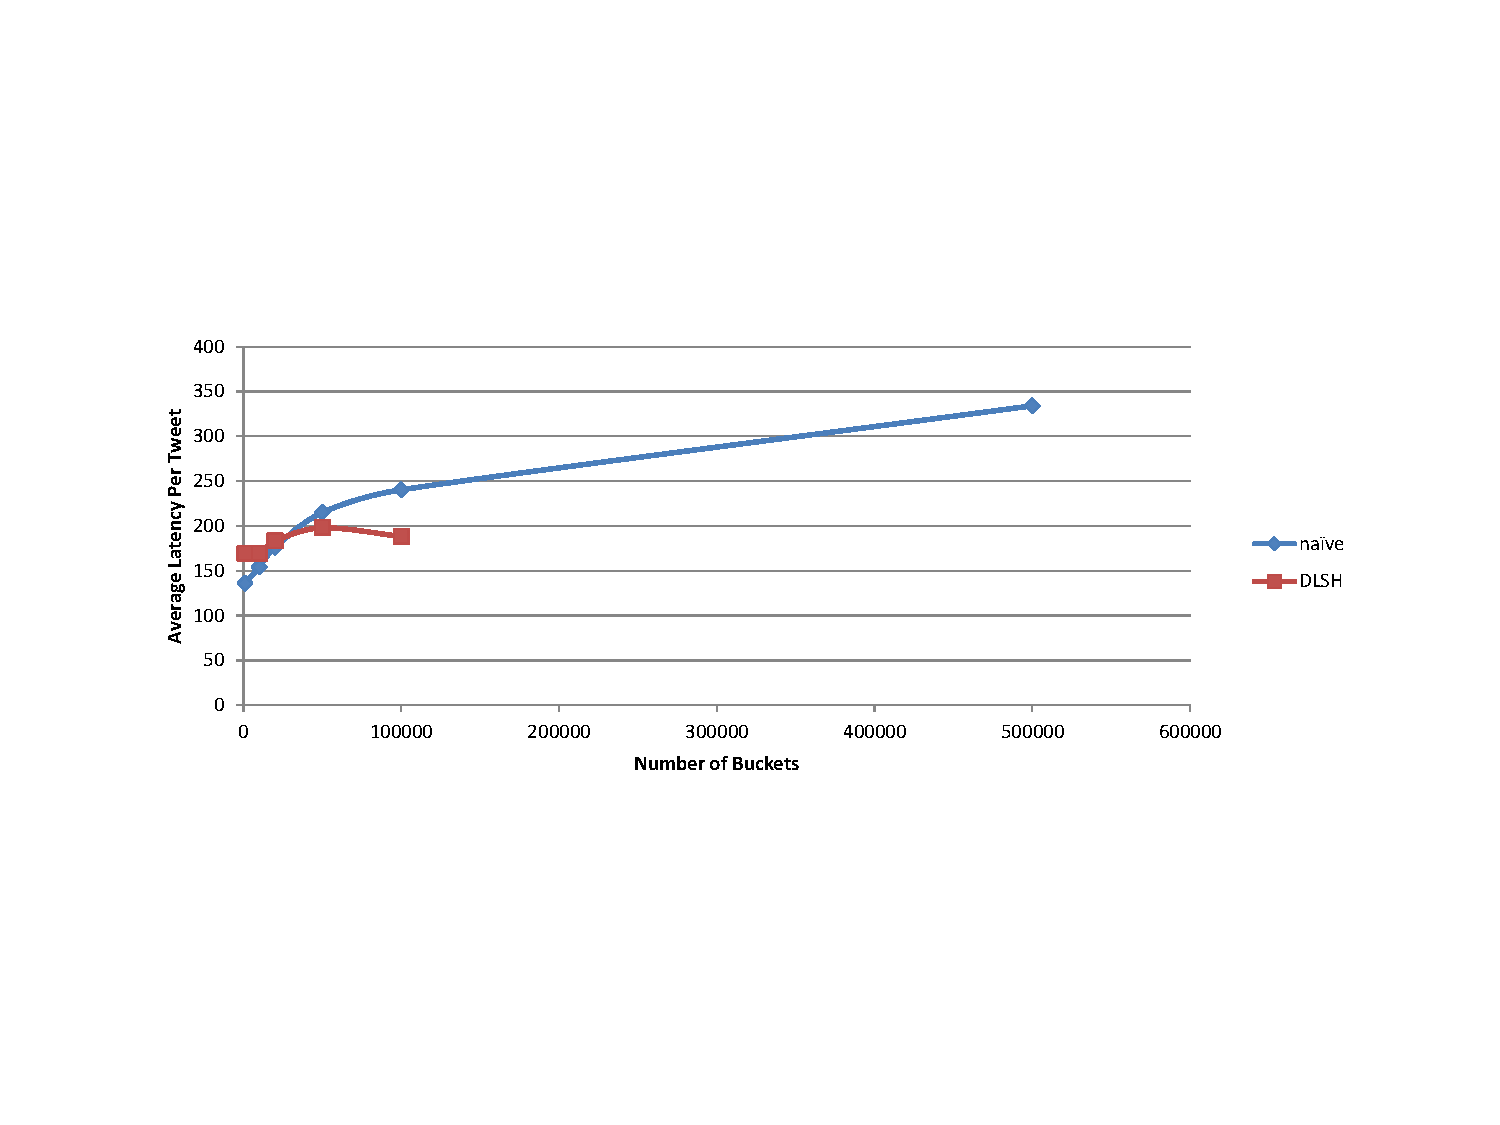
\includegraphics[width=0.8\columnwidth]{perf.pdf}
\caption{Average Latency Comparison: Naive Stream Clustering vs Distributed LSH Stream Clustering}
\label{fig:result}
\end{figure}

\section{Final Deliverables}
\label{sec:future}
\begin{enumerate}
\item Design improvements to be considered:
\begin{enumerate}
\item Bounding the number of buckets on each node.
\item Study other techniques to establish key representatives for a bucket instead of just a centroid to achieve better accuracy.
\end{enumerate}
\item Deploying on a true distributed system. ( Amazon EC2, if time permits )
\item Experimental analysis:
\begin{enumerate}
\item Effect of increasing data rates on performance ( latency ).
\item Analyse communication overhead.
\item Determine the resource requirements for desired performance characteristics.
\end{enumerate}
\end{enumerate}



\subsubsection*{References}

\small{

[1] 	Cheng Z., Caverlee J., Lee K., You Are Where You Tweet: A Content-Based Approach to Geo-locating Twitter Users. In Proceeding of the 19th ACM Conference on Information and Knowledge Management (CIKM), Toronto, Oct 2010. \newline
[2] Simmhan Y., Natarajan S., Kumbhare A., Prasanna V., Floe: Designing a Continuous Data Flow Engine for Dynamic Applications on the Cloud, tech report, University of Southern California (submitted). \newline
[3] Wadhwa, S.; Gupta, P.; , "Distributed Locality Sensitivity Hashing," Consumer Communications and Networking Conference (CCNC), 2010 7th IEEE , vol., no., pp.1-4, 9-12 Jan. 2010. \newline
<<<<<<< .mine
[4] Jure Leskovec, Lars Backstrom, Jon Kleinberg, Meme-tracking and the Dynamics of the News Cycle. ACM SIGKDD International Conference on Knowledge Discovery and Data Mining (ACM KDD), 2009. \newline
[5] B. Bahmani, A. Goel, R. Shinde. Efficient Distributed Locality Sensitive Hashing. To appear in CIKM 2012.
=======
[4] Jure Leskovec, Lars Backstrom, Jon Kleinberg, Meme-tracking and the Dynamics of the News Cycle. ACM SIGKDD International Conference on Knowledge Discovery and Data Mining (ACM KDD), 2009. \newline
[5] Daniel Barbara, Requirements for clustering data streams. ACM SIGKDD Explorations Newsletter Homepage archive
Volume 3 Issue 2, January 2002, Pages 23-27. \newline
[6] Madjid Khalilian, Norwati Mustapha, Data Stream Clustering: Challenges and Issues. Proceeding of the International MultiConference of Engineers and Computer Scienctists 2010 Vol I, IMECS 2010, March 17-19, 2010, Hong Kong. newline
>>>>>>> .r55
}

\end{document}
